\documentclass[xcolor={dvipsnames},aspectratio=169,compress]{beamer} % maybe 10pt?

%-------------------------------------------------------------------------------
%   REQUIRED PACKAGES AND SETTINGS
%-------------------------------------------------------------------------------
\usepackage[utf8]{inputenc}
\usepackage[T1]{fontenc}
\usepackage[english]{babel}
\usepackage{amsmath,amssymb}
\usepackage{booktabs}
\usepackage{graphicx}
\usepackage{pgfplots}
\pgfplotsset{compat=1.18}
\usepackage{pgfornament}
\usepackage{hyperref}
\usepackage{caption}
\usepackage{pifont}
\usepackage[p,osf,scaled=1.05]{erewhon}
\usepackage{fontawesome}
\usepackage{tikz}
\usepackage{tikzscale}
\usepackage{ifdraft}
\usepackage{csquotes}
\usepackage{subcaption}
\usepackage{bm}

\MakeOuterQuote{"}

% --- Font Setup ---
\usepackage[scaled=1.05]{zlmtt}
\usepackage[type1]{cabin}
\usepackage[utopia,vvarbb]{newtxmath}

\usepackage{../tikzviolinplots/tikzviolinplots}

% --- Tikz Setup ---
\usepgfplotslibrary{colorbrewer}
\usetikzlibrary{external,positioning,shapes,arrows.meta,calc,fit,shadows.blur,backgrounds}

% Set Cabin as the default sans-serif font
\renewcommand{\familydefault}{\sfdefault}

% Minted for code listings (NOTE: requires --shell-escape option during compilation)
\usepackage{minted}
\usemintedstyle{tango}
\setminted{
    fontsize=\footnotesize,
    breaklines,
    autogobble,
    frame=lines,
    framesep=2mm,
    rulecolor=\color{Gray!70},
    bgcolor=Gray!10
}

\newcommand{\follows}{\raisebox{-0.7mm}{\scalebox{1.4}{\textcolor{Maroon}{\ding{43}}}}}
\newcommand{\answer}[1]{\begin{description}\item[\follows{}]{#1}\end{description}}
\newcommand{\TODO}[1]{\textbf{\textcolor{red}{TODO: #1}}}
\newcommand{\glsentrylong}[1]{System Usability Scale}  % Only used in one included Tikz drawing for SUS

\newcommand{\plotornaments}[1]{
  \node[shift={(0.44,-0.47)}](CNW) at (#1.north west) {\pgfornament[color=Gray,width=1cm]{41}};
  \node[shift={(-0.44,-0.47)}](CNE) at (#1.north east) {\pgfornament[color=Gray,width=1cm,symmetry=v]{41}};
  \node[shift={(0.44,0.47)}](CSW) at (#1.south west) {\pgfornament[color=Gray,width=1cm,symmetry=h]{41}};
  \node[shift={(-0.44,0.47)}](CSE) at (#1.south east) {\pgfornament[color=Gray,width=1cm,symmetry=c]{41}};


  \draw[transform canvas={yshift=-1.8mm},line width=1pt,color=Gray] ([xshift=-1.5mm]CNW.north east) -- ([xshift=1.5mm]CNE.north west);
  \draw[transform canvas={yshift=1.8mm},line width=1pt,color=Gray] ([xshift=-1.5mm]CSW.south east) -- ([xshift=1.5mm]CSE.south west);
  \draw[transform canvas={xshift=2.05mm},line width=1pt,color=Gray] ([yshift=1.6mm]CNW.south west) -- ([yshift=-1.6mm]CSW.north west);
  \draw[transform canvas={xshift=-2.05mm},line width=1pt,color=Gray] ([yshift=1.6mm]CNE.south east) -- ([yshift=-1.6mm]CSE.north east);

    \begin{pgfonlayer}{axis ticks}
        \draw[white,thick] (#1.north west) -- (#1.north east);
        \draw[white,thick] (#1.south west) -- (#1.south east);
      \end{pgfonlayer}
}

\newcommand{\barplot}[3]{
\begin{tikzpicture}
  \begin{axis}[
      ylabel={Number of participants},
      height=5.5cm,
      ybar stacked,
      ytick distance=3,
      name=bars,
      set layers,
      ymin=0, ymax=16,
      axis x line*=bottom,
      axis y line*=left,
      ymajorgrids,
      bar width=0.6cm,
      symbolic x coords={#2},
      x tick label style={rotate=45, anchor=east, align=left, font=\scriptsize, yshift=-2},
      xtick=data,
      nodes near coords={\pgfmathprintnumber[precision=1]{\pgfplotspointmeta}},
      nodes near coords style={
          font=\scriptsize,
        },
      cycle list={
          {fill=Maroon!30,draw=Maroon!50!black,nodes near coords style={Maroon}},
          {fill=Gray,draw=black!70,nodes near coords style={white!50}},
        },
      #3
    ]

    \addplot+[fill] table [x=label,y=occ1,col sep=tab] {analysis/dat/#1.dat};
    \addplot+[fill] table [x=label,y=occ2,col sep=tab] {analysis/dat/#1.dat};
  \end{axis}
  \plotornaments{bars}
\end{tikzpicture}
}

\newcommand{\keystroke}[1]{%
  \tikz[baseline=(key.base)]
    \node[%
      draw,
      fill=gray!25,
      drop shadow={shadow xshift=0.25ex,shadow yshift=-0.25ex,fill=black,opacity=0.2},
      rectangle,
      rounded corners=2pt,
      inner ysep=0.5pt,
      inner xsep=3pt,
      line width=0.5pt,
      font=\footnotesize\sffamily
    ](key) {#1\strut}
  ;\hspace{-0.5ex}
}

\newcommand{\violin}[8]{
  \begin{tikzpicture}
    \violinsetoptions[data points,scaled,averages]{
      xmin=0,xmax=3,
      ymajorgrids=true,
      axis on top=false,
      set layers,
      name=violin,
      #5
    }

    \violinplot[%
      index=#4,%
      col sep=tab,%
      color=Maroon,%
      dataset size=3pt,%
      average size=5pt,%
      average opacity=0.8,%
      average color=black,%
      dataset opacity=0.8,%
      dataset jitter=0.1,%
      relative position=1,%
      average fill opacity=0.5,%
      average fill=ForestGreen,%
      average mark=otimes*,%
      bandwidth=#6,%
      dataset color=black,%
      dataset fill=black,%
      dataset fill opacity=0.5,%
      label={#2}
    ]{analysis/dat/\expandafter#1\expandafter#8.dat};

    \violinplot[%
      index=#4,%
      col sep=tab,%
      color=black,%
      dataset size=3pt,%
      average size=5pt,%
      average opacity=0.8,%
      average color=black,%
      average fill opacity=0.5,%
      average fill=ForestGreen,%
      average mark=otimes*,%
      bandwidth=#7,%
      dataset opacity=0.5,%
      dataset jitter=0.1,%
      relative position=2,%
      dataset fill=white,%
      dataset fill opacity=0.5,%
      label={#3}
    ]{analysis/dat/\expandafter#1\the\numexpr3-#8\relax.dat};

		\plotornaments{violin}
  \end{tikzpicture}
}

% 4key, options, ymin, ymax, bw1, bw2
\newcommand{\violinab}[7]{\violin{alphabeta}{$\Psi$}{$\Omega$}{#1}{ymin=#3,ymax=#4,#2}{#5}{#6}{#7}}
\newcommand{\violinsv}[7]{\violin{seevs}{SEE}{VSCode}{#1}{ymin=#3,ymax=#4,#2}{#5}{#6}{#7}}
\newcommand{\violinsus}{\violin{seevs-sus}{SEE}{VSCode}{sus}{ymin=40,ymax=100,ylabel=SUS}{7.4}{7.2153}{1}}

%-------------------------------------------------------------------------------
%   THEME CONFIGURATION
%-------------------------------------------------------------------------------

%\useoutertheme{miniframes}
\useoutertheme{split}
%\useoutertheme{sidebar}
\useinnertheme{rectangles}

% Apply colors
\setbeamercolor{palette primary}{bg=Maroon, fg=white}
\setbeamercolor{palette secondary}{bg=Maroon!85!black, fg=white}
\setbeamercolor{palette tertiary}{bg=Maroon!70!black, fg=white}
\setbeamercolor{palette quaternary}{bg=Maroon!50!black, fg=white}

\setbeamercolor{structure}{fg=Maroon}
\setbeamercolor{title}{fg=Maroon, bg=white}
\setbeamercolor{frametitle}{bg=Maroon!90!black, fg=white}
\setbeamercolor{sidebar}{bg=Maroon!90!black}
\setbeamercolor{sidebar text}{fg=white}
\setbeamercolor{section in sidebar}{fg=white}
\setbeamercolor{subsection in sidebar}{fg=white!80}
% \setbeamercolor{section in sidebar shaded}{fg=black!40}

\setbeamercolor{block title}{bg=Maroon!80, fg=white}
\setbeamercolor{block body}{bg=Maroon!10, fg=black}
\setbeamercolor{block title alerted}{bg=red!80!black, fg=white}
\setbeamercolor{block body alerted}{bg=red!10, fg=black}
\setbeamercolor{block title example}{bg=ForestGreen!80, fg=white}
\setbeamercolor{block body example}{bg=ForestGreen!10, fg=black}

% \setbeamercolor{normal text}{bg=white, fg=black}
% \setbeamercolor{item}{fg=Maroon}
% \setbeamercolor{subitem}{fg=Maroon!80}
% \setbeamercolor{subsubitem}{fg=Maroon!60}

\setbeamercolor{caption name}{fg=Maroon} % Figure/Table caption label
\setbeamercolor{author in head/foot}{fg=Gray, bg=white} % Footline colors
\setbeamercolor{title in head/foot}{fg=Gray, bg=white}
\setbeamercolor{date in head/foot}{fg=Gray, bg=white}
\setbeamercolor{page number in head/foot}{fg=Gray, bg=white}

\hypersetup{
    colorlinks=false,
    linkcolor=Fuchsia,
    citecolor=ForestGreen,
    urlcolor=Blue,
}

%-------------------------------------------------------------------------------
%   FONT CONFIGURATION
%-------------------------------------------------------------------------------

\usefonttheme{professionalfonts} % Allow font changes

% Set fonts for specific elements
% \setbeamerfont{title}{size=\LARGE, series=\bfseries}
% \setbeamerfont{subtitle}{size=\large}
% \setbeamerfont{author}{size=\normalsize}
% \setbeamerfont{institute}{size=\small}
% \setbeamerfont{date}{size=\small}
\setbeamerfont{frametitle}{size=\large, series=\bfseries}
\setbeamerfont{headline}{series=\scshape}
% \setbeamerfont{sidebar}{size=\tiny} % Smaller font in sidebar
% \setbeamerfont{section in sidebar}{size=\small, series=\bfseries}
% \setbeamerfont{subsection in sidebar}{size=\scriptsize}
% \setbeamerfont{footline}{size=\scriptsize}
\setbeamerfont{block title}{size=\normalsize, series=\bfseries}
\setbeamerfont{block body}{size=\small}
\setbeamerfont{caption}{size=\footnotesize}
\setbeamerfont{caption name}{series=\bfseries}

%-------------------------------------------------------------------------------
%   OUTER THEME CUSTOMIZATION
%-------------------------------------------------------------------------------

% \makeatletter
%   \setbeamertemplate{sidebar \beamer@sidebarside}%{sidebar theme}
%   {
%     \beamer@tempdim=\beamer@sidebarwidth%
%     \advance\beamer@tempdim by -6pt%
%     \insertverticalnavigation{\beamer@sidebarwidth}%
%     \vfill
%     \ifx\beamer@sidebarside\beamer@lefttext%
%     \else%
%       \usebeamercolor{normal text}%
%       \llap{\usebeamertemplate***{navigation symbols}\hskip0.1cm}%
%       \vskip2pt%
%     \fi%
%   }%
% \makeatother

% --- Navigation Symbols ---
\setbeamertemplate{navigation symbols}{} % Remove navigation symbols

% --- Footline ---
\setbeamertemplate{footline}[frame number]

%-------------------------------------------------------------------------------
%   INNER THEME CUSTOMIZATION
%-------------------------------------------------------------------------------

% --- Itemize ---
% Use standard triangles, colored with structure color
\setbeamertemplate{itemize item}{\color{Maroon}\raise0.5pt\hbox{\tiny$\blacksquare$}} % Use tiny square
\setbeamertemplate{itemize subitem}{\color{Maroon!80}\raise0.5pt\hbox{\tiny$\blacksquare$}}
\setbeamertemplate{itemize subsubitem}{\color{Maroon!60}\raise0.5pt\hbox{\tiny$\blacksquare$}}

% --- Enumerate ---
\setbeamertemplate{enumerate item}{\insertenumlabel.}
\setbeamertemplate{enumerate subitem}{\insertenumlabel.\insertsubenumlabel}
\setbeamertemplate{enumerate subsubitem}{\insertenumlabel.\insertsubenumlabel.\insertsubsubenumlabel}

\setbeamersize{description width=0.5cm}

% Increase separation between items
\let\OLDitemize\itemize
\renewcommand\itemize{\OLDitemize\addtolength{\itemsep}{0.5em}}

% Set colors for title page elements (some might be inherited)
\setbeamercolor{title}{fg=Maroon, bg=white}
\setbeamercolor{subtitle}{fg=black, bg=white}
% \setbeamercolor{author}{fg=black, bg=white}
% \setbeamercolor{institute}{fg=Gray, bg=white}
% \setbeamercolor{date}{fg=Gray, bg=white}
\setbeamercolor{logo}{bg=white} % Ensure logo background is white if needed
%\setbeamercolor{subsection in sidebar shaded}{fg=black!40} % Explicitly set shaded subsection color

%-------------------------------------------------------------------------------
%   BIBLIOGRAPHY SETUP
%-------------------------------------------------------------------------------
% Use Beamer's built-in bibliography item style
\setbeamertemplate{bibliography item}{\insertbiblabel}
%\setlength{\bibsep}{1em}

%-------------------------------------------------------------------------------
%   PRESENTATION METADATA
%-------------------------------------------------------------------------------
\title{Building Code Cities using the Language Server Protocol}
\subtitle{Master's Thesis Presentation}
\author{Falko Galperin}
\institute[Uni Bremen]{%
  %Working group Software Engineering \\
  Faculty 3---Mathematics \& Computer Science \\
  University of Bremen
}
\titlegraphic{
\includegraphics[height=0.6cm]{figures/unibremen}}
\date{\today}

%-------------------------------------------------------------------------------
%   PRESENTATION CONTENT STARTS HERE
%-------------------------------------------------------------------------------


\begin{document}

{
\begin{frame}[plain,noframenumbering]
	\titlepage
\end{frame}
}

\section{Introduction}

\begin{frame}{Outline}
	\tableofcontents
\end{frame}

\begin{frame}{Overview}
	\begin{itemize}
		\item \textbf{Code Cities} can help developers understand complex software systems
		      \begin{itemize}
			      \item Often limited to few languages
		      \end{itemize}
		\item The \textbf{Language Server Protocol} (LSP) specifies how \emph{Language Servers} can provide language-specific features to IDEs
		      \begin{itemize}
			      \item Many Language Servers are available
		      \end{itemize}
	\end{itemize}
	\begin{block}{Goal}
		\answer{Integrate LSP information into code-city implementation SEE}
	\end{block}

	% TODO: Images (e.g., explanatory LSP/SEE graphic)

\end{frame}

\begin{frame}{Research Questions}
	\begin{alertblock}{Research Question 1}
		How can LSP be integrated into SEE to generate code cities?
	\end{alertblock}

	\begin{exampleblock}{Research Question 2}
		What is the scalability of this integration?
	\end{exampleblock}

	\begin{block}{Research Question 3}
		Are code cities a suitable means to present LSP information to developers as compared to IDEs + tables (on the dimensions of speed, accuracy, and usability)?
	\end{block}
\end{frame}

\begin{frame}{SEE: Graph}
	Attributed project graph $G = (V, E, a, s, t, \ell)$

	\begin{itemize}
		\item $V$: Set of nodes
		\item $E$: Set of edges
		\item $a: (V \times \mathcal{A}_K) \rightharpoonup \mathcal{A}_V$ assigns named attributes to nodes
		\item $s, t: E \rightarrow V$ denotes source/target node of each edge
		\item $\ell: E \rightarrow \Sigma$ for labelling edges
		      \begin{itemize}
			      \item Edge label $\texttt{partOf} \in \Sigma$ induces source code hierarchy
		      \end{itemize}
	\end{itemize}
\end{frame}

\begin{frame}{Language Server Protocol}
	\begin{itemize}
		\item Open-source specification managed by Microsoft
		\item JSON-RPC messages sent between Language Client and Language Server
		\item $>260$ Language Servers, $>60$ Language Clients
		\item Specifies \textbf{capabilities} to be used by implementers
		      \begin{itemize}
			      \item Examples: Go to definition, hover, document symbols
			      \item We will only use (some) "read-only" capabilities
		      \end{itemize}
	\end{itemize}
\end{frame}
%

\section{Implementation}

\subsection{Algorithm}

\begin{frame}{Part I: Node Synthesis}
	\ifdraft{Omitted in draft}{
		\centering
		\includegraphics{figures/tikz/algorithm_pres1.tikz}
	}
\end{frame}

\begin{frame}{Part II: Edge Synthesis}
	\ifdraft{Omitted in draft}{
		\centering
		\includegraphics{figures/tikz/algorithm_pres2.tikz}
	}
\end{frame}

\begin{frame}{Part III: Aggregation}
	\ifdraft{Omitted in draft}{
		\centering
		\includegraphics{figures/tikz/algorithm_pres3.tikz}
	}

\end{frame}

% TODO: Note performance problems / augmented interval trees in any way?
% \begin{frame}{Augmented Interval Trees}
% 	Left out
% \end{frame}

\subsection{Integration}

\begin{frame}{Code Cities}
	\begin{figure}
		\begin{center}
			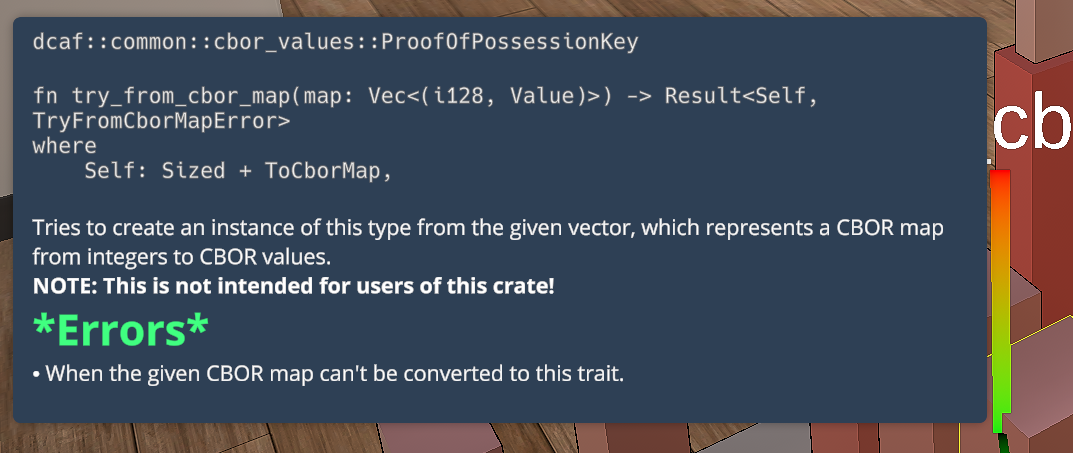
\includegraphics[trim={0.3cm 0.8cm 2.7cm 0.3cm},clip,width=0.95\textwidth]{figures/HoverInfo}
		\end{center}
		\caption{A hover tooltip with information collected from the \texttt{rust-analyzer} Language Server.}
	\end{figure}

\end{frame}

\begin{frame}{Code Windows}
	\begin{figure}
		\begin{center}
			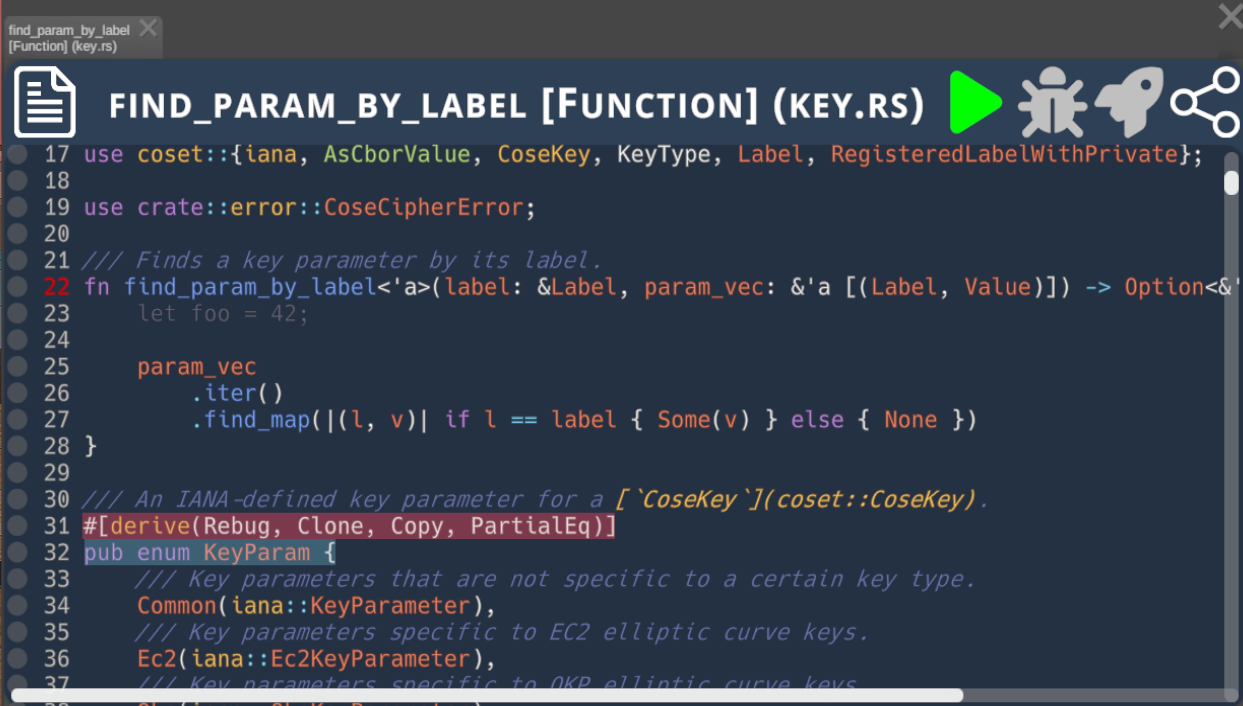
\includegraphics[width=0.8\textwidth]{figures/CodeWindow}
		\end{center}
		\caption{A code window with enabled LSP integration.}
	\end{figure}
\end{frame}

\begin{frame}{Generating Cities}
	\begin{columns}
		\column{0.5\linewidth}
		\begin{figure}
			\begin{center}
				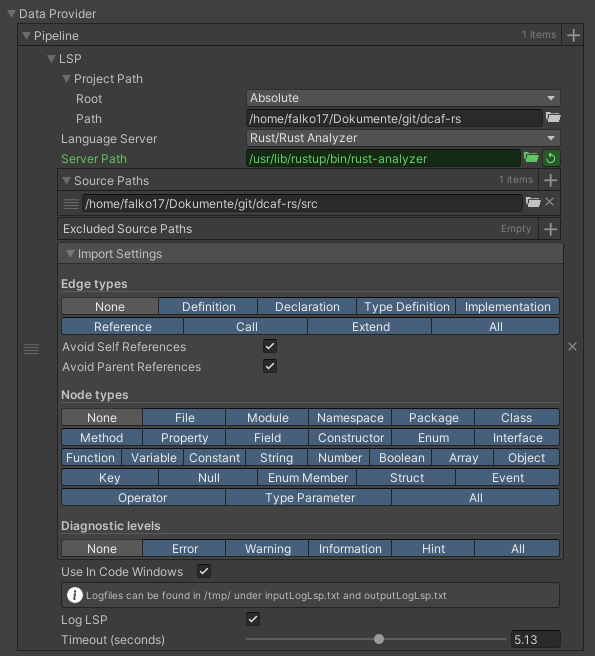
\includegraphics[height=6.5cm]{figures/unity_lsp_provider}
			\end{center}
			\caption{Unity Editor UI for the LSP graph provider.}
		\end{figure}

		\column{0.45\linewidth}
		\begin{alertblock}{Research Question 1}
			\emph{How can LSP be integrated into SEE to generate code cities?}
			\answer{\small Answered in previous slides}
		\end{alertblock}
	\end{columns}

\end{frame}

\subsection{Technical Evaluation}

\begin{frame}{Evaluation Setup}
	\begin{itemize}
		\item Ran generation algorithm on six projects in total: two per Java, Rust, \LaTeX{}
		\item Measured average execution time across multiple runs
		\item \emph{Only} generation algorithm included in measurement
		      \begin{itemize}
			      \item E.\,g., no layouting or visual rendering of nodes
		      \end{itemize}
		\item Later followed up in paper submitted to ICSME~2025
	\end{itemize}
\end{frame}

\begin{frame}[plain]{Evaluation Results---Time Breakdown}

	\begin{figure}
		\begin{subfigure}[T]{0.5\textwidth}
			\begin{center}
				\begin{tikzpicture}
					\begin{axis}[
							ylabel={Time in seconds},
							height=6.5cm,
							ybar stacked,
							name=bars,
							set layers,
							ymin=0, ymax=370,
							axis line style={draw=none},
							enlarge x limits={0.5},
							ymajorgrids,
							bar width=0.6cm,
							x tick label style={rotate=45, anchor=east, align=left, font=\scriptsize, yshift=-2},
							xtick=data,
							width=\textwidth,
							xticklabels={\proptt{aaoffline}-$O$, \proptt{aaoffline}-$B$, \proptt{dcaf-rs}-$O$, \proptt{dcaf-rs}-$B$},
							xtick={0,1,3,4},
							legend entries={Nodes, Edges, Diagnostics, Aggregation, Tree Creation, Miscellaneous},
							legend style={nodes={scale=0.7, transform shape}, at={(0.5,0.9)}}
						]

						\addplot+[fill] table [x=index,y=LSP Nodes,col sep=tab] {benchmark/rust.dat};
						\addplot+[fill] table [x=index,y=LSP Edges,col sep=tab] {benchmark/rust.dat};
						\addplot+[fill] table [x=index,y=LSP Diagnostics,col sep=tab] {benchmark/rust.dat};
						\addplot+[fill] table [x=index,y=LSP Aggregate,col sep=tab] {benchmark/rust.dat};
						\addplot+[fill] table [x=index,y=LSP Tree,col sep=tab] {benchmark/rust.dat};
						\addplot+[fill] table [x=index,y=LSP Miscellaneous,col sep=tab] {benchmark/rust.dat};
					\end{axis}
					\plotornaments{bars}
				\end{tikzpicture}
			\end{center}
		\end{subfigure}
		\begin{subfigure}[T]{0.49\textwidth}
			\begin{center}
				\begin{tikzpicture}
					\begin{axis}[
							height=6.5cm,
							ybar stacked,
							name=bars,
							set layers,
							ymin=0, ymax=2700,
							axis line style={draw=none},
							axis y line*=left,
							xmin=3, xmax=4,
							enlarge x limits={1},
							ymajorgrids,
							bar width=0.6cm,
							x tick label style={rotate=45, anchor=east, align=left, font=\scriptsize, yshift=-2},
							xtick=data,
							width=\textwidth,
							xticklabels={SpotBugs-$O$, SpotBugs-$B$},
							xtick={3,4},
						]

						\addplot+[fill] table [x=index,y=LSP Nodes,col sep=tab] {benchmark/java.dat};
						\addplot+[fill] table [x=index,y=LSP Edges,col sep=tab] {benchmark/java.dat};
						\addplot+[fill] table [x=index,y=LSP Diagnostics,col sep=tab] {benchmark/java.dat};
						\addplot+[fill] table [x=index,y=LSP Aggregate,col sep=tab] {benchmark/java.dat};
						\addplot+[fill] table [x=index,y=LSP Tree,col sep=tab] {benchmark/java.dat};
						\addplot+[fill] table [x=index,y=LSP Miscellaneous,col sep=tab] {benchmark/java.dat};
					\end{axis}
					\plotornaments{bars}
				\end{tikzpicture}
			\end{center}
		\end{subfigure}
		\caption{Generation time for Rust and \LaTeX{} projects, broken down by parts of the algorithm.
			The suffix \emph{O} denotes the optimized version of the algorithm, while \emph{B} refers to the brute-force version.
		}
	\end{figure}
\end{frame}

\begin{frame}[plain]{Evaluation Results---Optimization Improvement}
	\begin{figure}
		\begin{center}
			\begin{tikzpicture}[
					labelnode/.style={font=\footnotesize,Maroon}
				]
				\begin{semilogxaxis}[
						height=6.5cm,
						name=line,
						set layers,
						ymin=0, ymax=1,
						xmin=10^(2.7), xmax=55000,
						xtick distance=10^(0.5),
						xtick distance=10^(0.5),
						axis line style={draw=none},
						grid=major,
						xlabel={Number of edges},
						ylabel={Relative time improvement},
						width=\textwidth,
					]

					\addplot+[draw=black,
						mark=*,
						mark options={fill=Maroon,draw=Maroon},
						% nodes near coords,
						% nodes near coords align={above left},
						% every node near coord/.append style={font=\footnotesize,Maroon},
						point meta=explicit symbolic,
						ultra thick,
						error bars/.cd,
						y dir=both,y explicit,
					] table [meta=project,x=edges,y=adv_mean,y error minus=adv_min,y error plus=adv_max,col sep=tab] {benchmark/advantage.dat};


					\node[labelnode] at (axis cs: 10^2.87,0.08) {JabRef};
					\node[labelnode] at (axis cs: 10^2.97,0.29) {\proptt{aaoffline}};
					\node[labelnode] at (axis cs: 10^3.9,0.29) {\proptt{dcaf-rs}};
					\node[labelnode] at (axis cs: 10^4.1,0.82) {SpotBugs};
					\node[labelnode] at (axis cs: 10^4.4,0.68) {Master's thesis};
					\node[labelnode] at (axis cs: 10^4.45,0.95) {Bachelor's thesis};
				\end{semilogxaxis}
				\plotornaments{line}
			\end{tikzpicture}
		\end{center}
		\caption{The percentage by which time is reduced when using the optimized instead of the base algorithm.}
	\end{figure}
\end{frame}

\begin{frame}{Evaluation Results---Conclusion}
	\begin{itemize}
		\item Time taken only comparable within the same Language Server
		\item Most important metric by far: Number of edges
		\item Optimized variant always more performant than brute-force approach
		      \begin{itemize}
			      \item $\mathcal{O}(|E| \cdot \log |V|)$ vs.\ $\Theta(|E| \cdot |V|)$
		      \end{itemize}
	\end{itemize}

	\begin{exampleblock}{Research Question 2}
		\emph{What is the scalability of this integration?}
		\answer{\small Feasible until $\approx 200$ kLOC (but very dependent on configuration and Language Server)}
	\end{exampleblock}
\end{frame}

\section{User Study}

\subsection{Design}

\begin{frame}{Plan}
	\begin{columns}
		\column{0.5\textwidth}
		\begin{itemize}
			\item User study comparing SEE + LSP with VSCode + LSP
			\item Most LSP capabilities are hard to evaluate
			      \answer{\small Hence, we focus on the generated city itself}
		\end{itemize}

		\column{0.5\textwidth}
		We measure five dependent variables:
		\begin{enumerate}
			\item \textbf{Correctness}
			\item \textbf{Speed}
			\item \textbf{Usability}, differentiating between:
			      \begin{enumerate}
				      \item \textbf{SUS} (post-study)
				      \item \textbf{ASQ} (post-task), measuring:
				            \begin{enumerate}
					            \item Perceived \textbf{complexity}
					            \item Perceived \textbf{effort}
				            \end{enumerate}
			      \end{enumerate}
		\end{enumerate}
	\end{columns}
\end{frame}

\begin{frame}{VSCode}
	\begin{figure}
		\begin{center}
			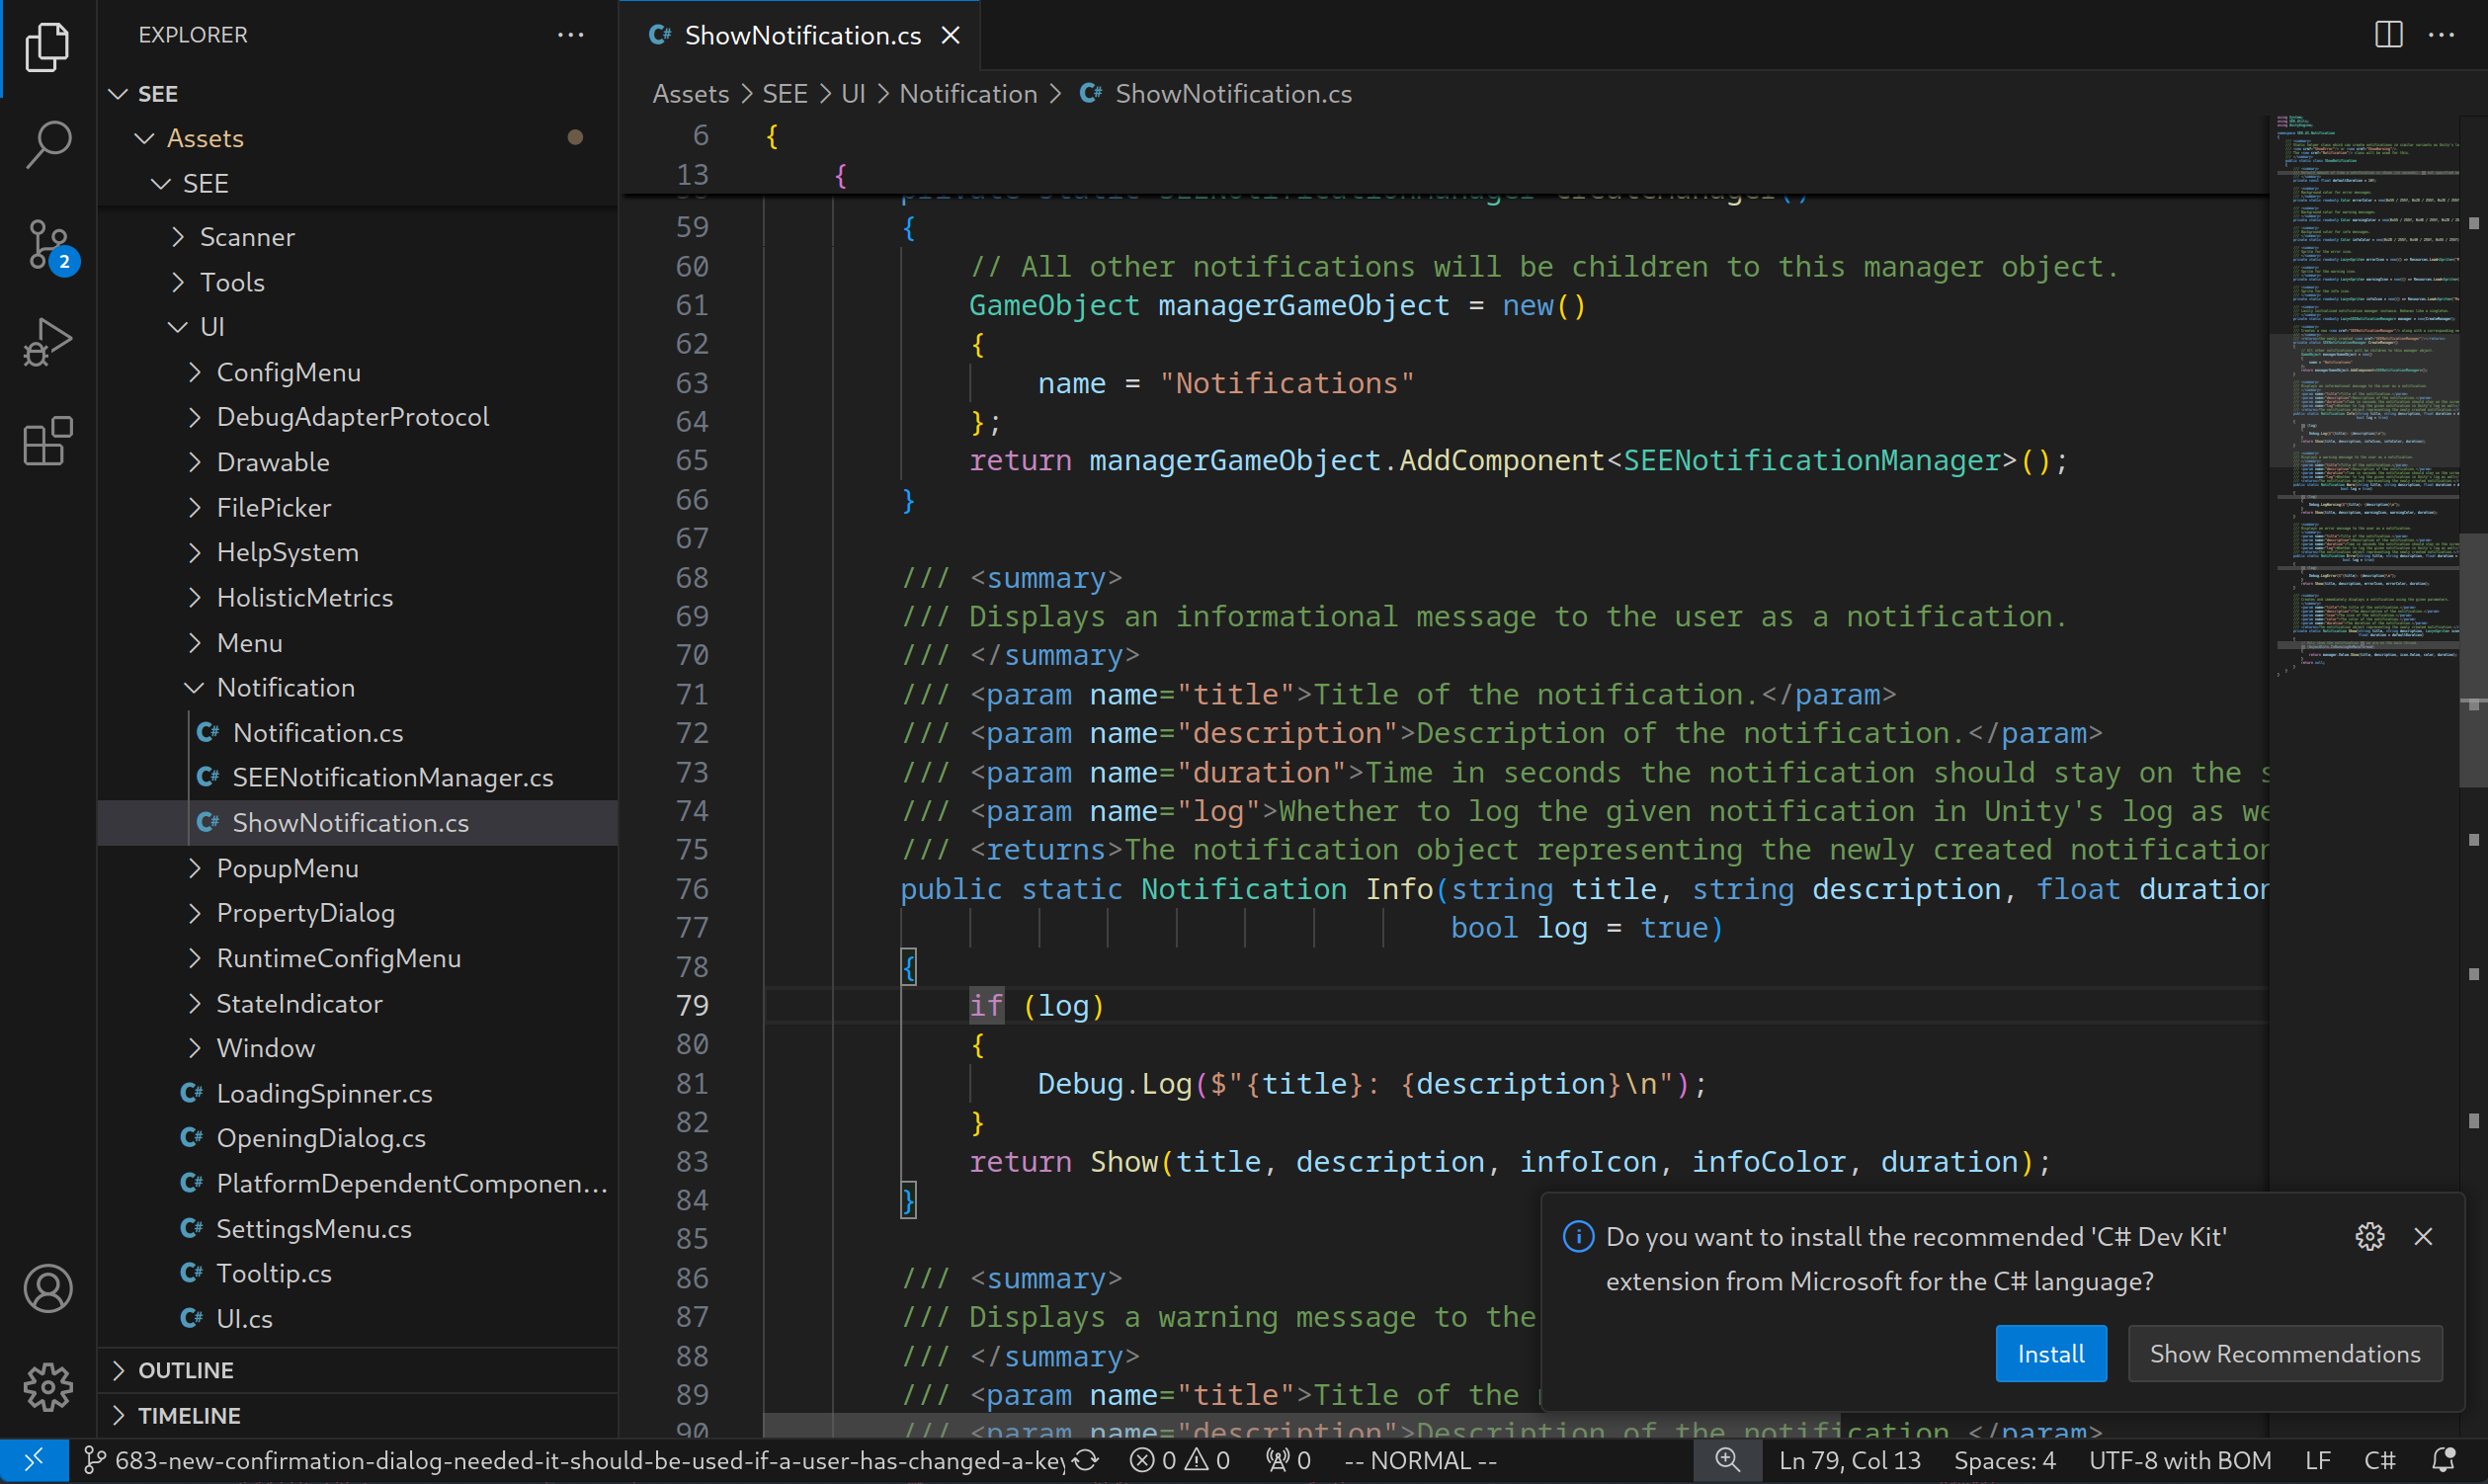
\includegraphics[width=0.75\textwidth]{figures/VSCode.png}
		\end{center}
		\caption{Screenshot of the main UI of VSCode.}
	\end{figure}

\end{frame}

\begin{frame}{Tasks}
	\begin{columns}

		\column{0.6\linewidth}
		\vspace{-0.3cm}
		\begin{figure}
			\begin{center}
				\scalebox{0.5}{
					\includegraphics{figures/tikz/taskflow.tikz}
				}
			\end{center}
		\end{figure}

		\column{0.5\linewidth}
		\begin{itemize}
			\item Within-subject study
			\item Three tasks per condition
			\item \emph{JabRef} and \emph{SpotBugs} used as object~systems
			\item ASQ after each task
			\item SUS after each condition
		\end{itemize}
	\end{columns}

\end{frame}

\subsection{Results}

\begin{frame}{Study Results}
	\begin{columns}
		\column{0.5\linewidth}
		\begin{itemize}
			\item $N = 19$ participants
			\item Significance level of $\alpha = 0.05$
			\item Used \emph{Mann-Whitney $U$ test} as statistical test (with some exceptions)
		\end{itemize}

		\column{0.5\linewidth}
		\begin{figure}
			\caption{"How long have you been programming?"}
			\barplot{alphabeta-programming}{Less than 3 years, 3–9 years, 10–19 years}{width=\textwidth, ylabel={},enlarge x limits={0.7}}
		\end{figure}
	\end{columns}

\end{frame}

\begin{frame}{Correctness}
	\begin{itemize}
		\item Answers manually checked for correctness (to catch, e.\,g., misspellings)
		\item \emph{Fisher's exact test} used due to binary results
		\item No significant differences for any of the tasks
	\end{itemize}
\end{frame}

\begin{frame}{Time}
	\begin{itemize}
		\item Time measured automatically
		\item Only correct answers included in analysis
		\item \alert{Significant differences} for task $C$ (reach base class) in favor of VSCode
		      \answer{\small Potential cause: following edges in SEE requires more navigation/interaction than just repeatedly \keystroke{Ctrl}-clicking in VSCode}
	\end{itemize}
\end{frame}

% \begin{frame}{Time: Significant Differences}
% 	\ifoptionfinal{
% 		\begin{figure}
% 			\begin{subfigure}[T]{0.5\textwidth}
% 				\includegraphics[width=\textwidth,height=6cm]{figures/tikz/a3t.tikz}
% 				\caption{Time taken for task $C_1$.}
% 			\end{subfigure}\hfill
% 			\begin{subfigure}[T]{0.5\textwidth}
% 				\includegraphics[width=\textwidth,height=6cm]{figures/tikz/a6t.tikz}
% 				\caption{Time taken for task $C_2$.}
% 			\end{subfigure}
% 		\end{figure}}{\TODO{Specify final option to see}}
% \end{frame}

\begin{frame}{Usability: ASQ}
	\begin{itemize}
		\item Two questions asked after each task
		\item "Cognitive" complexity: No significant differences for any task
		\item "Temporal" effort: \alert{Significant differences} for tasks $A_2$ and $C_1$ in favor of VSCode
		      \begin{itemize}
			      \item Participants indeed took longer to solve tasks $A_2$ and $C_1$ in SEE
		      \end{itemize}
	\end{itemize}
\end{frame}

\begin{frame}{Usability: SUS}
	\begin{columns}
		\column{0.55\textwidth}
		\begin{figure}
			\center
			\ifoptionfinal{\violinsus}{\TODO{Specify final option to see}}
		\end{figure}

		\column{0.4\textwidth}
		\begin{itemize}
			\item Ten questions asked about each system
			\item \emph{Wilcoxon signed-rank test} used due to dependent samples
			\item \alert{Significant difference} in favor of VSCode
			      \begin{itemize}
				      \item SUS score falls in line with previous usability experiments involving SEE
			      \end{itemize}
		\end{itemize}
	\end{columns}
\end{frame}

\begin{frame}{The Effects of Experience}
	\begin{itemize}
		\item We want to find correlations between independent and dependent variables
		      \begin{itemize}
			      \item Especially to check if, e.\,g., experience may bias our results
		      \end{itemize}
		\item \emph{Kendall's coefficient of rank correlation $\tau_b$} used as statistical test
		      \begin{itemize}
			      \item However, at 90 tests, we run into the multiple comparisons problem
			      \item Hence, \emph{Benjamini-Yekutieli procedure} used to fix False Discovery Rate at $0.05$
		      \end{itemize}
		\item Result: No significant correlations for any pair of variables (after FDR correction)
	\end{itemize}
\end{frame}

\begin{frame}{The Effects of Experience---Heatmap}
	\begin{figure}
		\begin{center}
			\scalebox{0.8}{\includegraphics{figures/tikz/corr.tikz}}
		\end{center}
		\caption{Correlations ($\tau_b$) between independent and dependent variables.
			Dependent variables for SEE are marked in \textcolor{Maroon}{red} and those for VSCode in \textcolor{Gray!50!black}{gray}.}
	\end{figure}
\end{frame}

\begin{frame}{Summary}
	\vspace{-0.3cm}
	\begin{table}
		\caption{Significant differences between the variables, all in favor of {VSCode}.}
		\centering
		\begin{tabular}{@{}lcccccc@{}}
			\toprule
			\textbf{Variable}        & $\bm{A_1}$                              & $\bm{B_1}$ & $ \bm{C_1}$        & $\bm{A_2}$          & $\bm{B_2}$ & $\bm{C_2}$         \\\midrule
			\emph{Correctness}       & ---                                     & ---        & ---                & ---                 & ---        & ---                \\
			\emph{Time}              & ---                                     & ---        & $p \approx 0.0015$ & ---                 & ---        & $p \approx 0.0247$ \\
			\emph{{ASQ}: Complexity} & ---                                     & ---        & ---                & ---                 & ---        & ---                \\
			\emph{{ASQ}: Effort}     & ---                                     & ---        & $p \approx 0.0142$ & $p \approx 0.00531$ & ---        & ---                \\
			\emph{{SUS}}             & \multicolumn{6}{c}{$p \approx 0.02116$}                                                                                           \\
			\bottomrule
		\end{tabular}
	\end{table}

	\begin{block}{Research Question 3}
		\emph{Are code cities a suitable means to present LSP information to developers as compared to IDEs + tables (on the dimensions of speed, accuracy, and usability)?}
		\answer{While code cities seem suitable to present LSP information, developers work faster and prefer traditional IDEs (at least in the case of SEE vs.\ VSCode).}
	\end{block}
\end{frame}

\section{Conclusion}

% \begin{frame}{Summary}
%
% 	\begin{alertblock}{Research Question 1}
% 		\emph{How can LSP be integrated into SEE to generate code cities?}
% 		\answer{\small Using the algorithm explained in previous slides}
% 	\end{alertblock}
%
% 	\begin{exampleblock}{Research Question 2}
% 		\emph{What is the scalability of this integration?}
% 		\answer{\small Feasible until $\approx 200$ kLOC (but very dependent on configuration and Language Server)}
% 	\end{exampleblock}
%
% 	\begin{block}{Research Question 3}
% 		\emph{Are code cities a suitable means to present LSP information to developers as compared to IDEs + tables (on the dimensions of speed, accuracy, and usability)?}
% 		\answer{While code cities seem suitable to present LSP information, developers work faster and prefer traditional IDEs (at least in the case of SEE vs.\ VSCode).}
% 	\end{block}
% \end{frame}

\begin{frame}{Future Work}
	\begin{itemize}
		\item Improve performance to make it possible for bigger projects to run well
		\item Add suport for editing-related capabilities to SEE
		\item Use the Language Server Index Format (LSIF) to construct code cities remotely
		\item Utilize a registry to automatically download and set up Language Servers in SEE
	\end{itemize}
\end{frame}


\begin{frame}{Thank You!}
	\vspace{1cm}
	\centering
	\Large Any questions?
	\vspace{1cm}

	\vfill
	
\begin{tikzpicture}
		\node[color=Maroon!80] {\pgfornament[width=7cm]{88}};
	\end{tikzpicture}

	{\footnotesize \url{https://github.com/falko17/masterthesis}}
\end{frame}

\appendix

\ifdraft{
	\begin{frame}{TODOs: General}
		\begin{itemize}
			\item Explain performance improvements (interval tree) in any way?
			\item Gradual blend-in of new content on some slides
		\end{itemize}
	\end{frame}

	\begin{frame}{TODOs: Appendix}
		\begin{itemize}
			\item Bibliography
			\item Full Algorithm
		\end{itemize}
	\end{frame}
}

\end{document}
